\documentclass[12pt,a4paper]{report}

% ---------- Packages ----------
\usepackage[margin=1in]{geometry}
\usepackage[T1]{fontenc}
\usepackage{lmodern}
\usepackage{graphicx}
\usepackage{xcolor}
\usepackage{booktabs}
\usepackage{tabularx}
\usepackage{array}
\usepackage{enumitem}
\usepackage{fancyhdr}
\usepackage{listings}
\usepackage{caption}
\usepackage{tikz}
\usetikzlibrary{arrows.meta, positioning, shapes.geometric, fit, calc}
\usepackage[colorlinks=true,linkcolor=black,urlcolor=blue]{hyperref}

\setlength{\headheight}{15pt}
\setlength{\parindent}{0pt}
\setlength{\parskip}{6pt}
\renewcommand{\arraystretch}{1.25}

% ---------- Placeholders: search the .tex for "fillin" before submitting ----------
\newcommand{\fillin}[1]{\textbf{#1}}

% ---------- Screenshot helper: shows a box until the image file exists ----------
% Usage: \screenshot{images/dashboard.png}{Caption text}{0.85}
\newcommand{\screenshot}[3]{%
  \begin{figure}[htbp]
    \centering
    \IfFileExists{#1}{%
      \includegraphics[width=#3\textwidth]{#1}%
    }{%
      \fbox{\parbox[c][6cm][c]{0.8\textwidth}{\centering\textcolor{red}{Screenshot missing:\\\texttt{#1}}}}%
    }
    \caption{#2}
  \end{figure}%
}

% ---------- Code listings ----------
\lstset{
  basicstyle=\ttfamily\small,
  frame=single,
  breaklines=true,
  columns=fullflexible,
  keepspaces=true,
  backgroundcolor=\color{gray!8},
  numbers=none
}

% ---------- Header / footer ----------
\pagestyle{fancy}
\fancyhf{}
\fancyhead[L]{UCS503 - Software Engineering}
\fancyhead[R]{PatchWatch \quad \thepage}
\renewcommand{\headrulewidth}{0.4pt}
\fancypagestyle{plain}{%
  \fancyhf{}
  \fancyfoot[C]{\thepage}
  \renewcommand{\headrulewidth}{0pt}
}

% ---------- TikZ styles ----------
\tikzset{
  box/.style={draw, rounded corners=3pt, align=center, minimum height=9mm, minimum width=28mm, fill=blue!6},
  ext/.style={draw, rounded corners=3pt, align=center, minimum height=9mm, minimum width=28mm, fill=orange!12},
  store/.style={draw, cylinder, shape border rotate=90, aspect=0.25, align=center, minimum height=12mm, minimum width=24mm, fill=green!10},
  flow/.style={draw, rounded corners=3pt, align=center, minimum height=8mm, text width=7.5cm, fill=blue!6},
  arr/.style={-{Stealth[length=2.5mm]}, thick},
  uc/.style={draw, ellipse, align=center, font=\small, minimum height=8mm, inner sep=1pt, fill=white}
}

\begin{document}

% =====================================================================
% TITLE PAGE
% =====================================================================
\begin{titlepage}
  \centering
  \vspace*{1cm}
  {\Large UCS503 - Software Engineering\par}
  \vspace{1.5cm}
  {\Huge\bfseries PatchWatch\par}
  \vspace{0.5cm}
  {\Large Software Dependency Security and Risk Dashboard\par}
  \vspace{2cm}

  {\large\bfseries Submitted by:\par}
  \vspace{0.3cm}
  \begin{tabular}{ll}
    \fillin{1024030004} & \fillin{Diya Gupta} \\
    \fillin{1024030007} & \fillin{Durva Garg} \\
    \fillin{1024030010} & \fillin{Mysha Bansal} \\
  \end{tabular}\par
  \vspace{0.5cm}
  Group: \fillin{3C11} \quad B.E.\ \fillin{3rd Year}, COE\par

  \vspace{1.5cm}
  {\large\bfseries Submitted to:\par}
  \vspace{0.3cm}
  \fillin{Ms. Paramveer Kaur}\par
  \vspace{0.3cm}
  \fillin{Prototype Evaluation}\par

  \vfill
  Computer Science and Engineering Department\par
  Thapar Institute of Engineering and Technology, Patiala
\end{titlepage}

\pagenumbering{roman}
\tableofcontents
\clearpage
\pagenumbering{arabic}

% =====================================================================
% CHAPTER 1
% =====================================================================
\chapter{Introduction}

\section{Background and Context}
Almost no modern web application is written from scratch. A typical JavaScript project pulls in dozens of direct dependencies from npm, and each of those pulls in more. Every one of these packages is code the developer did not write and usually has not read. When a security flaw is found in one of them, it is published in a public vulnerability database, but nothing forces the developer to find out. In practice the project keeps running with a known-vulnerable version until someone happens to notice.

The data needed to catch this already exists. OSV.dev is an open vulnerability database that can be queried by package name and version. What is missing for a student or small team is a simple tool that takes the dependency list they already have, checks it, and presents the result in a form that shows what is risky and what to fix first.

PatchWatch is a web application built for that gap. A user uploads a \texttt{package.json}, the backend extracts the dependencies, each one is checked against OSV.dev, the findings are stored in a database, and a dashboard shows the severity breakdown, a risk score, the vulnerable packages, and the version that fixes each problem.

\section{Motivation}
In the Software Engineering course we had to choose a real problem and build it the way a software team would: a proposal, design diagrams, incremental implementation, and testing. Dependency vulnerabilities are a problem every one of us runs into as soon as we use \texttt{npm install}, so the topic was easy to relate to. We also wanted a project where the core feature talks to a real external service instead of a hard-coded demo. The work was approached collaboratively across interface design, backend development, integration, documentation, and testing. The frontend and backend were developed in parallel where possible, then integrated so that scan results from the API could be displayed by the dashboard.

\section{Problem Statement}
Developers do not have a quick, visual way to learn which of their project's dependencies have known vulnerabilities. Checking by hand means looking up every package in a database, which does not scale. Raw scanner output is also hard to act on because it does not say which issue to fix first. There is no history either, so a team cannot tell whether the project is getting safer or riskier over time.

\section{Project Objectives}
The status of each objective is stated as it is in the code today, not as it was planned.
\begin{enumerate}[leftmargin=*]
  \item Let a user upload a \texttt{package.json} and extract its runtime and development dependencies. 
  \item Check every dependency against the live OSV.dev API and normalize the severity of each finding. 
  \item Persist each scan and its findings in a database so that results survive a server restart and scan history is available. 
  \item Present the results on a dashboard with summary cards, a severity-coded dependency table, priority fixes, a risk score, and a scan-history chart. 
  \item Provide user accounts and multiple projects. 
  \item License analysis, outdated-version detection, and \texttt{package-lock.json} / \texttt{requirements.txt} support. 
\end{enumerate}

% =====================================================================
% CHAPTER 2
% =====================================================================
\chapter{Methodology and Design}

\section{Overall Approach}
We followed an iterative and incremental model. Instead of building all of the frontend, then all of the backend, we built one working vertical slice at a time and made each slice run end to end before starting the next. The intended order was: a frontend that runs, a minimal backend API, one frontend feature connected to the backend, database persistence, the scanner, and then the connection of scanning, database, API, and dashboard.

One consequence of this approach was that the frontend team was able to work ahead of the backend. The login, registration, and project management screens were built against a mocked layer so the interface could be completed while the backend only supported scanning. The mock is isolated in two files and documented in the code, so it can be replaced by real endpoints later without changing the pages that use it.

\begin{table}[htbp]
\centering
\begin{tabularx}{\textwidth}{>{\raggedright\arraybackslash}p{2cm} X}
\toprule
\textbf{Phase} & \textbf{What was built} \\
\midrule
1 & Repository skeleton, frontend UI prototype (dashboard layout, stat cards, sample vulnerability table with hard-coded data) \\
2 & FastAPI application with root and health endpoints; \texttt{package.json} parser \\
3 & OSV.dev integration (\texttt{vuln\_checker}); first real scan end to end \\
4 & SQLite persistence with SQLAlchemy models; scan history endpoints \\
5 & Frontend rebuilt in React with routing; dashboard driven by real scan data; mocked auth and projects \\
6 & Automated tests, one-click start scripts, documentation \\
\bottomrule
\end{tabularx}
\caption{Build phases in implementation order. The table records the sequence of work rather than calendar dates.}
\end{table}

\section{System Architecture}

\subsection{High-Level Design}
PatchWatch has three parts: a React frontend that runs in the browser, a FastAPI backend that owns all data and business logic, and an external vulnerability source, OSV.dev. The browser never contacts OSV.dev directly; it only talks to our backend. This keeps the external call, the error handling, and the severity normalization in one place.

\begin{figure}[htbp]
\centering
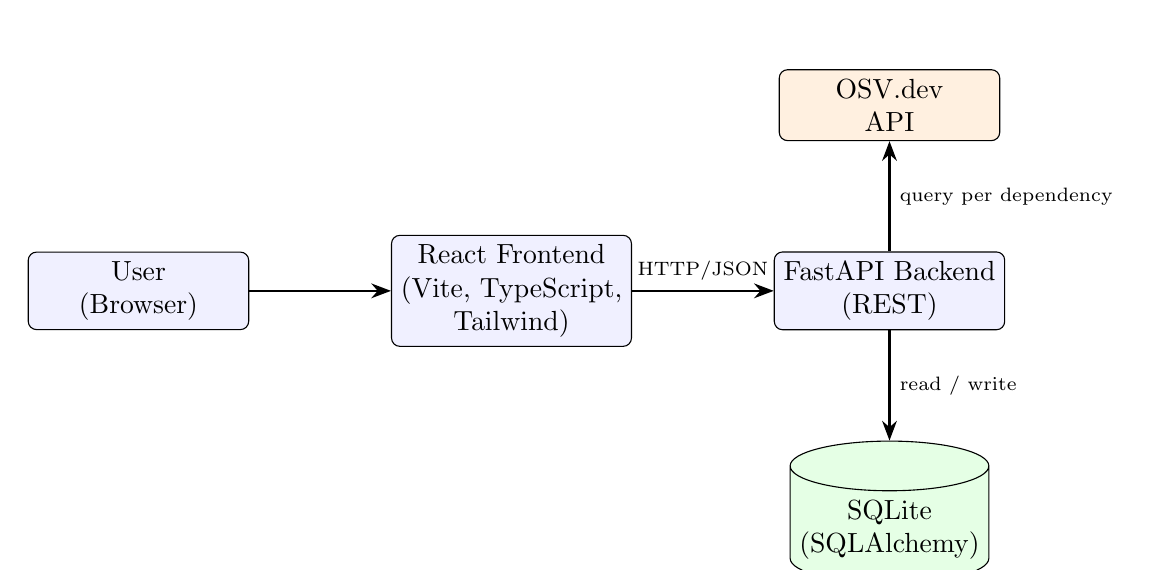
\begin{tikzpicture}[node distance=14mm and 18mm]
  \node[box] (user) {User\\(Browser)};
  \node[box, right=of user] (fe) {React Frontend\\(Vite, TypeScript,\\Tailwind)};
  \node[box, right=of fe] (be) {FastAPI Backend\\(REST)};
  \node[store, below=of be] (db) {SQLite\\(SQLAlchemy)};
  \node[ext, above=of be] (osv) {OSV.dev\\API};
  \draw[arr] (user) -- (fe);
  \draw[arr] (fe) -- node[above, font=\scriptsize]{HTTP/JSON} (be);
  \draw[arr] (be) -- node[right, font=\scriptsize]{read / write} (db);
  \draw[arr] (be) -- node[right, font=\scriptsize]{query per dependency} (osv);
\end{tikzpicture}
\caption{High-level architecture of PatchWatch.}
\end{figure}

\subsection{Request Flow when a User Runs a Scan}
Unlike a background-job design, a scan in PatchWatch is processed inside a single request: the upload does not return until every dependency has been checked and the result is stored. This is acceptable for the size of a typical \texttt{package.json} because the OSV lookups are issued concurrently, and the frontend allows up to 60 seconds for the response.

\begin{figure}[htbp]
\centering
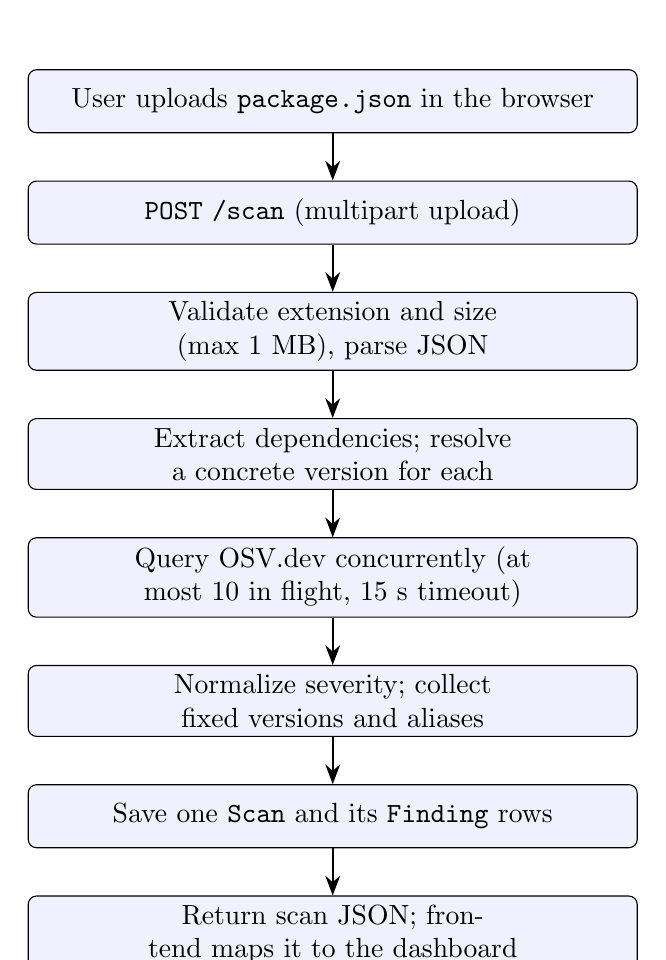
\begin{tikzpicture}[node distance=6mm]
  \node[flow] (a) {User uploads \texttt{package.json} in the browser};
  \node[flow, below=of a] (b) {\texttt{POST /scan} (multipart upload)};
  \node[flow, below=of b] (c) {Validate extension and size (max 1 MB), parse JSON};
  \node[flow, below=of c] (d) {Extract dependencies; resolve a concrete version for each};
  \node[flow, below=of d] (e) {Query OSV.dev concurrently (at most 10 in flight, 15 s timeout)};
  \node[flow, below=of e] (f) {Normalize severity; collect fixed versions and aliases};
  \node[flow, below=of f] (g) {Save one \texttt{Scan} and its \texttt{Finding} rows};
  \node[flow, below=of g] (h) {Return scan JSON; frontend maps it to the dashboard};
  \foreach \i/\j in {a/b,b/c,c/d,d/e,e/f,f/g,g/h} \draw[arr] (\i) -- (\j);
\end{tikzpicture}
\caption{Request flow for a scan.}
\end{figure}

\section{Technical Stack}
\begin{itemize}[leftmargin=*]
  \item \textbf{Backend:} Python 3.10+, FastAPI, Uvicorn, SQLAlchemy 2.0, httpx (async HTTP client), python-multipart.
  \item \textbf{Database:} SQLite, created automatically on first run.
  \item \textbf{Frontend:} React 19, TypeScript, Vite, Tailwind CSS 4, React Router, Axios, lucide-react icons.
  \item \textbf{External data source:} OSV.dev vulnerability API (npm ecosystem).
  \item \textbf{Testing:} pytest with FastAPI's \texttt{TestClient}.
  \item \textbf{Tooling:} Git and GitHub for version control; \texttt{start.bat} / \texttt{start.sh} scripts that install dependencies and launch both servers.
\end{itemize}

\section{UML Use Case Diagram}
Because accounts exist only in the browser at this stage, there is a single actor, the user (a developer). OSV.dev is shown as an external system the backend depends on.

\begin{figure}[htbp]
\centering
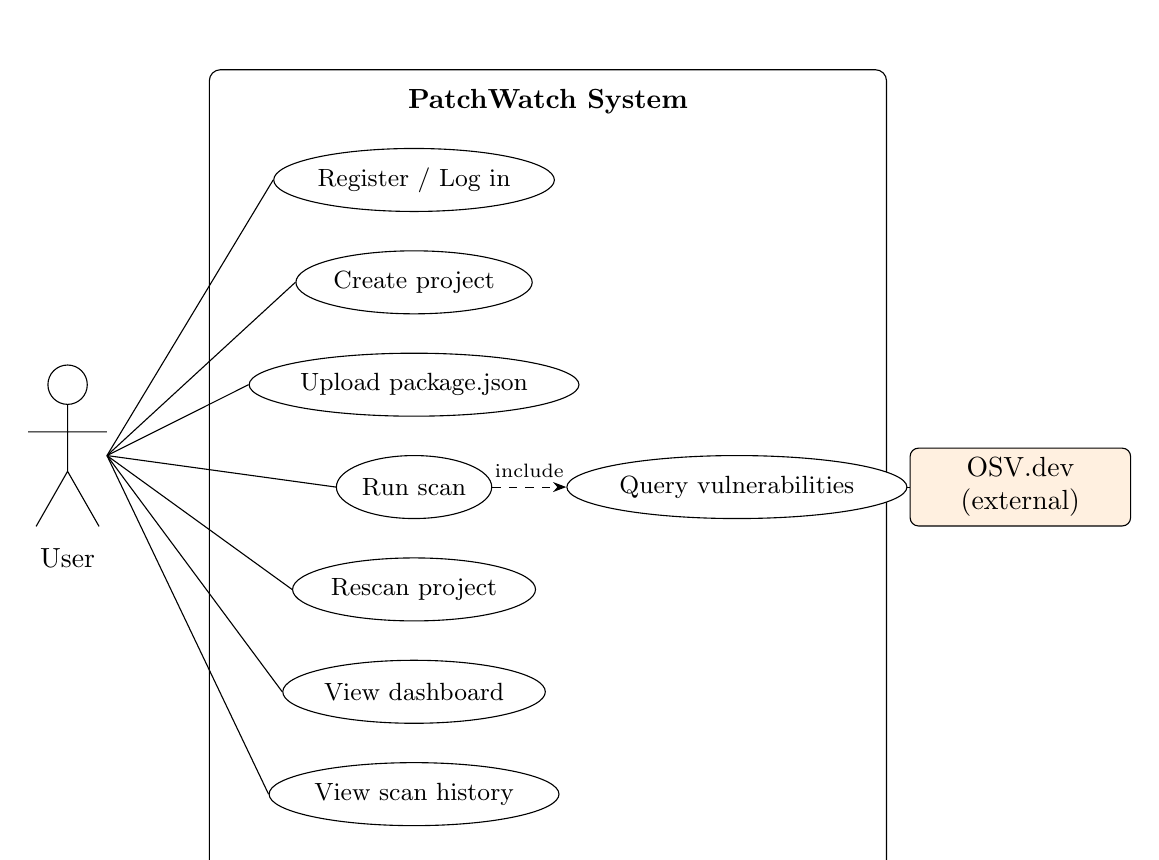
\begin{tikzpicture}[x=1cm,y=1cm]
  \draw[rounded corners] (2.6,-0.6) rectangle (11.2,9.6);
  \node[font=\bfseries] at (6.9,9.2) {PatchWatch System};

  % actor: user
  \draw (0.8,5.6) circle (0.25);
  \draw (0.8,5.35) -- (0.8,4.5) (0.3,5.0) -- (1.3,5.0) (0.8,4.5) -- (0.4,3.8) (0.8,4.5) -- (1.2,3.8);
  \node at (0.8,3.4) {User};

  % use cases
  \node[uc] (u1) at (5.2,8.2) {Register / Log in};
  \node[uc] (u2) at (5.2,6.9) {Create project};
  \node[uc] (u3) at (5.2,5.6) {Upload package.json};
  \node[uc] (u4) at (5.2,4.3) {Run scan};
  \node[uc] (u5) at (5.2,3.0) {Rescan project};
  \node[uc] (u6) at (5.2,1.7) {View dashboard};
  \node[uc] (u7) at (5.2,0.4) {View scan history};
  \node[uc] (u8) at (9.3,4.3) {Query vulnerabilities};

  \foreach \n in {u1,u2,u3,u4,u5,u6,u7} \draw (1.3,4.7) -- (\n.west);
  \draw[dashed,-{Stealth}] (u4.east) -- node[above,font=\scriptsize]{include} (u8.west);

  % external actor
  \node[ext] (osvact) at (12.9,4.3) {OSV.dev\\(external)};
  \draw (u8.east) -- (osvact.west);
\end{tikzpicture}
\caption{Use case diagram of PatchWatch.}
\end{figure}

\section{Data Model}
The database has two tables. A \texttt{Scan} stores the summary of one upload, and each \texttt{Finding} stores one vulnerability found for one package version in that scan. Deleting a scan deletes its findings.

\begin{figure}[htbp]
\centering
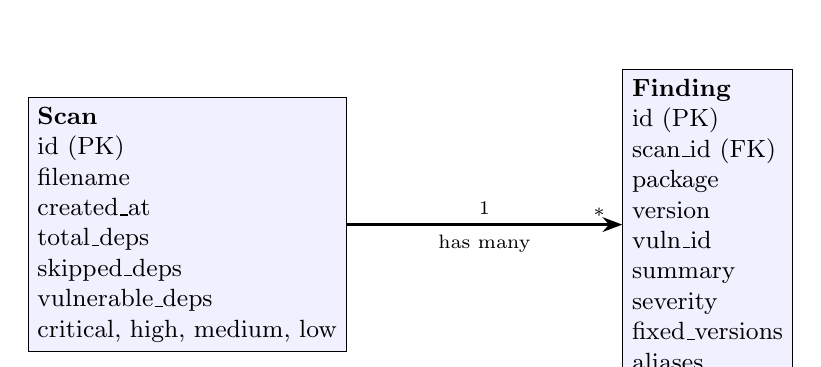
\begin{tikzpicture}
  \node[draw, align=left, font=\small, fill=blue!6] (scan) {%
    \textbf{Scan}\\
    id (PK)\\ filename\\ created\_at\\ total\_deps\\ skipped\_deps\\ vulnerable\_deps\\ critical, high, medium, low};
  \node[draw, align=left, font=\small, fill=blue!6, right=3.5cm of scan] (find) {%
    \textbf{Finding}\\
    id (PK)\\ scan\_id (FK)\\ package\\ version\\ vuln\_id\\ summary\\ severity\\ fixed\_versions\\ aliases};
  \draw[arr] (scan.east) -- node[above,font=\scriptsize]{1} node[below,font=\scriptsize]{has many} (find.west);
  \node[font=\scriptsize, above left=-1mm and 1mm of find.west] {*};
\end{tikzpicture}
\caption{Entity--relationship diagram.}
\end{figure}

\section{Dependency Check States}
Each dependency in the uploaded file ends up in exactly one of four states. This is what lets the system report \emph{why} a dependency was not checked instead of silently ignoring it.

\begin{figure}[htbp]
\centering
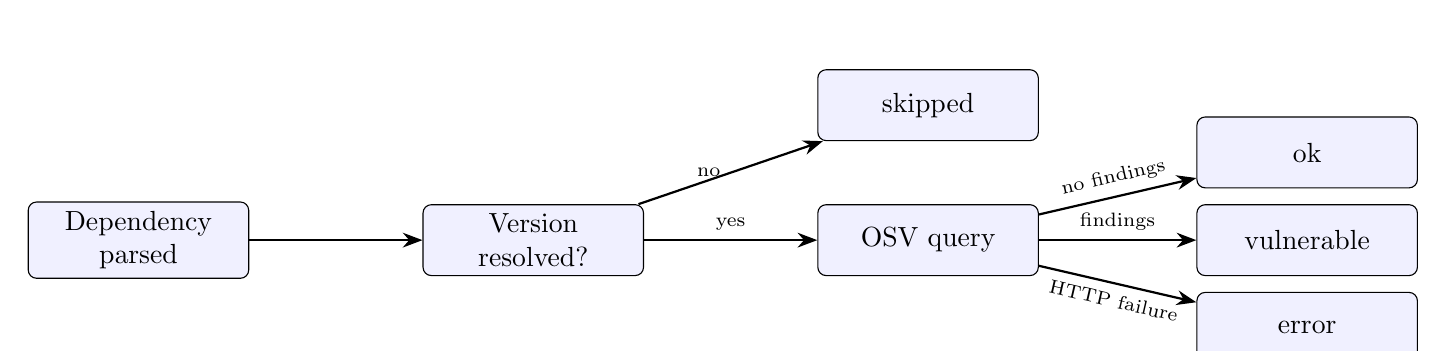
\begin{tikzpicture}[node distance=14mm and 22mm]
  \node[box] (dep) {Dependency\\parsed};
  \node[box, right=of dep] (res) {Version\\resolved?};
  \node[box, above right=8mm and 22mm of res] (skip) {skipped};
  \node[box, right=of res] (q) {OSV query};
  \node[box, above right=2mm and 20mm of q] (ok) {ok};
  \node[box, right=20mm of q] (vul) {vulnerable};
  \node[box, below right=2mm and 20mm of q] (err) {error};
  \draw[arr] (dep) -- (res);
  \draw[arr] (res) -- node[left,font=\scriptsize]{no} (skip);
  \draw[arr] (res) -- node[above,font=\scriptsize]{yes} (q);
  \draw[arr] (q) -- node[above,font=\scriptsize,sloped]{no findings} (ok);
  \draw[arr] (q) -- node[above,font=\scriptsize]{findings} (vul);
  \draw[arr] (q) -- node[below,font=\scriptsize,sloped]{HTTP failure} (err);
\end{tikzpicture}
\caption{States a dependency can end in after a scan.}
\end{figure}

\section{Risk Score Design}
The backend returns findings and counts but does not compute a risk score. The frontend computes a 0--100 score from the real findings. Each finding is given points according to its severity, and the overall score is the mean of those points.

\begin{table}[htbp]
\centering
\begin{tabular}{lc}
\toprule
\textbf{Severity} & \textbf{Points} \\
\midrule
Critical & 90 \\
High & 70 \\
Medium & 45 \\
Low & 20 \\
Unknown & 10 \\
\bottomrule
\end{tabular}
\qquad
\begin{tabular}{lc}
\toprule
\textbf{Score range} & \textbf{Category} \\
\midrule
0--24 & Low \\
25--49 & Moderate \\
50--74 & High \\
75--100 & Critical \\
\bottomrule
\end{tabular}
\caption{Severity points and risk categories (frontend heuristic).}
\end{table}

This is a heuristic, and we label it as one in the code. Section~\ref{sec:limits} discusses its weakness.

% =====================================================================
% CHAPTER 3
% =====================================================================
\chapter{Implementation}

\section{Backend}
The backend is a FastAPI application in \texttt{backend/app/}. The entry point \texttt{main.py} creates the tables on startup, enables CORS so the frontend on port 5173 can call the API on port 8000, and defines the routes. \texttt{models.py} holds the SQLAlchemy models, \texttt{database.py} creates the engine and the per-request session, and the \texttt{services/} folder holds the parsing and vulnerability-checking logic.

\subsection{API Endpoints}
\begin{table}[htbp]
\centering
\begin{tabularx}{\textwidth}{>{\ttfamily}l X}
\toprule
\textbf{Endpoint} & \textbf{Purpose} \\
\midrule
GET /health & Liveness check \\
POST /scan & Upload a \texttt{package.json}, check it, store and return the result \\
GET /scans & List all scans (summary only), newest first \\
GET /scans/\{id\} & One scan with all of its findings \\
DELETE /scans/\{id\} & Delete a scan and its findings \\
GET /stats & Summary numbers of the latest scan \\
GET /api/scan & Parser-only check using the bundled sample file \\
\bottomrule
\end{tabularx}
\caption{Backend API.}
\end{table}

The upload endpoint rejects files that do not end in \texttt{.json} (HTTP 400), files over 1 MB (HTTP 413), and content that is not valid JSON (HTTP 400).

\subsection{Parser}
\texttt{parser.py} reads both \texttt{dependencies} and \texttt{devDependencies} and marks each entry as development or runtime. npm version specifiers such as \verb|^4.17.15| or \verb|~1.2| cannot be sent to OSV as they are, so \texttt{clean\_version} converts them to a single concrete version. Specifiers that cannot be resolved (\texttt{*}, \texttt{latest}, git and file URLs) return \texttt{None} and the dependency is reported as skipped.

\begin{lstlisting}[language=Python, caption={Version cleaning in \texttt{parser.py}.}]
def clean_version(spec: str) -> str | None:
    if not isinstance(spec, str):
        return None
    if spec.startswith(("git", "http", "file:", "link:", "workspace:")):
        return None
    m = _VERSION_RE.search(spec)
    if not m:
        return None
    major, minor, patch, pre = m.groups()
    return f"{major}.{minor or 0}.{patch or 0}{pre or ''}"
\end{lstlisting}

For a range such as \verb|^4.16.0| this returns the lowest version the range allows, which is an approximation because no lockfile is available.

\subsection{Vulnerability Checker}
\texttt{vuln\_checker.py} sends one POST request per dependency to the OSV query endpoint with the package name, the npm ecosystem, and the version. The requests run concurrently with \texttt{asyncio.gather}, and a semaphore limits the number in flight to 10 so that a large dependency list does not flood the API. Each request has a 15-second timeout. A network or HTTP error for one package is recorded as that package's error and does not abort the scan.

For each vulnerability returned, the checker extracts the identifier, summary, aliases (such as CVE numbers), the fixed versions for that package, and a severity. GitHub advisories carry a plain severity label, which is read and normalized: \texttt{MODERATE} is mapped to \texttt{MEDIUM}, and anything unrecognized becomes \texttt{UNKNOWN}.

\begin{lstlisting}[language=Python, caption={Concurrent checking in \texttt{vuln\_checker.py}.}]
async def check_all_dependencies(dependencies: list[dict]) -> list[dict]:
    sem = asyncio.Semaphore(MAX_CONCURRENT)
    async with httpx.AsyncClient(timeout=15.0) as client:
        return await asyncio.gather(
            *(_check_one(client, sem, d) for d in dependencies)
        )
\end{lstlisting}

\subsection{Persistence}
After checking, the \texttt{/scan} handler builds one \texttt{Scan} row with the counts per severity and one \texttt{Finding} row per vulnerability, then commits both in a single transaction. Fixed versions and aliases are stored as comma-separated strings and split back into lists when the scan is serialized.

\section{Frontend}
The frontend is a single-page React application with the following routes.

\begin{table}[htbp]
\centering
\begin{tabularx}{\textwidth}{>{\ttfamily}l X}
\toprule
\textbf{Route} & \textbf{Page} \\
\midrule
/login, /register & Authentication screens (mocked, see below) \\
/projects & List of the user's projects; create a new project \\
/projects/:projectId/upload & Drag-and-drop upload of \texttt{package.json} and Run scan \\
/dashboard/:projectId & Risk score, summary cards, priority fixes, dependency table, scan history \\
\bottomrule
\end{tabularx}
\caption{Frontend routes.}
\end{table}

Reusable components include the risk score card, stat cards, dependency table, priority fix list, risk history chart, file dropzone, severity badges, and a modal for creating a project. Pages other than login and register are wrapped in a \texttt{ProtectedRoute} that redirects unauthenticated users to the login page.

\texttt{scanApi.ts} contains the real backend calls through Axios. \texttt{mapScanToDashboard.ts} converts the backend's scan response into the shape the dashboard displays, groups findings by package and version, sorts packages by risk, selects the three most severe findings as priority fixes, and computes the risk score described in Section~2.7. Values the backend cannot provide (license, latest version, outdated status) are shown as unknown instead of being invented.

\textbf{Mocked layer.} Registration, login, and projects are stored in the browser's \texttt{localStorage} through \texttt{authService.ts} and \texttt{mockData.ts}. Passwords in this mock are not hashed and the tokens are not verified by any server; this layer exists only so the interface could be built and demonstrated before backend authentication exists.

\screenshot{login.jpeg}{Login screen.}{0.7}
\screenshot{project.jpeg}{Projects page.}{0.8}
\screenshot{upload.jpeg}{Upload page with a dropped \texttt{package.json}.}{0.8}
\screenshot{dashboard.jpeg}{Dashboard after a real scan: risk score, summary cards, priority fixes, and dependency table.}{0.95}
\screenshot{history.jpeg}{Scan history chart after a rescan.}{0.8}

\section{Running the Project}
\texttt{start.bat} (Windows) and \texttt{start.sh} (macOS/Linux) create the Python virtual environment, install backend and frontend dependencies, start Uvicorn on port 8000 and Vite on port 5173, and open the browser. The \texttt{stop} scripts shut both servers down. The repository includes \texttt{sample\_package.json}, which contains deliberately old versions of \texttt{lodash} and \texttt{minimist} so that a demonstration scan produces findings.

% =====================================================================
% CHAPTER 4
% =====================================================================
\chapter{Results and Testing}

\section{Testing Strategy}
Testing was kept practical and was split into two levels.
\begin{itemize}[leftmargin=*]
  \item \textbf{Automated backend tests (pytest).} Parser tests check version cleaning and the runtime/development split. API tests run against an in-memory SQLite database. They replace the OSV call with a fake so the tests are fast and do not need a network connection.
  \item \textbf{Manual end-to-end checks.} Because the automated tests mock OSV.dev, the real integration was checked by hand against the live API, using the sample file and the running frontend.
\end{itemize}

\section{Automated Test Results}
All four automated tests pass (\texttt{4 passed}).

\begin{table}[htbp]
\centering
\begin{tabularx}{\textwidth}{c >{\raggedright\arraybackslash}p{4.8cm} X c}
\toprule
\textbf{\#} & \textbf{Test} & \textbf{What it checks} & \textbf{Result} \\
\midrule
1 & \texttt{test\_clean\_version} & \verb|^4.17.15|, \verb|~1.2|, \verb|>=2| resolve to concrete versions; \texttt{*}, \texttt{latest}, and git URLs return \texttt{None} & Pass \\
2 & \texttt{test\_parse\_includes\_dev} & Both dependency sections are parsed and dev dependencies are flagged & Pass \\
3 & \texttt{test\_scan\_saves\_and\_lists} & Upload saves a scan; list, detail, and stats endpoints return it; delete removes it and a second lookup returns 404 & Pass \\
4 & \texttt{test\_bad\_json\_rejected} & Invalid JSON upload returns HTTP 400 & Pass \\
\bottomrule
\end{tabularx}
\caption{Automated test results.}
\end{table}

\section{Manual End-to-End Test Plan}

\begin{table}[htbp]
\centering
\small
\begin{tabularx}{\textwidth}{c >{\raggedright\arraybackslash}p{3.4cm} X}
\toprule
\textbf{\#} & \textbf{Test case} & \textbf{Expected behaviour to verify during the demonstration} \\
\midrule
1 & Scan \texttt{sample\_package.json} & The scan completes and the dashboard displays findings and severity counts returned by the live OSV.dev service. Record actual counts and elapsed time during the run. \\
2 & Upload a file with no known vulnerable dependencies & The scan completes and reports no vulnerability findings for the checked versions. \\
3 & Upload a non-JSON file or invalid JSON & The API rejects the upload with an appropriate error; invalid JSON is expected to return HTTP 400. \\
4 & Dependency with \texttt{*} or a git URL & The dependency is marked as skipped because a concrete version cannot be resolved by the parser. \\
5 & Run without internet access & Network failures should be recorded as dependency-level errors where handled by the checker; verify that the application does not terminate unexpectedly. \\
6 & Restart the backend and reload scan history & Previously saved scan records should remain available because the application persists scans in SQLite. \\
7 & Rescan the same project & A new scan should be saved and, if the frontend history chart is connected to the returned scan history, a new history point should appear. \\
\bottomrule
\end{tabularx}
\caption{Manual end-to-end test plan and expected behaviour. Actual outcomes must be recorded after execution.}
\end{table}

\section{Discussion}\label{sec:limits}
The central feature works: a real dependency file is parsed, checked against live data, stored, and displayed. We also want to state the limitations plainly.

\begin{enumerate}[leftmargin=*]
  \item \textbf{Version resolution is approximate.} Without a lockfile, a range like \verb|^4.16.0| is checked as \texttt{4.16.0}, the lowest version it allows. The version npm would actually install may be newer and may not be affected. The scan can therefore over-report for ranges, and it cannot see the transitive dependencies at all.
  \item \textbf{The risk score can mislead.} It is the average of per-finding points, so adding a low-severity finding to a project that already has a critical one lowers the score. A weighted or maximum-based score would be more defensible. Since it is computed in the browser, it is also not stored with the scan.
  \item \textbf{Authentication and projects are not real.} They live in \texttt{localStorage}. The backend has no users, so every scan is global and any client can list or delete any scan. The CORS policy currently allows all origins. This is acceptable for a local demo and not for deployment.
  \item \textbf{Automated tests do not cover OSV.dev.} The live integration, the severity extraction on real responses, and the frontend are only checked manually. There are no frontend tests.
  \item \textbf{Single page of OSV results.} The checker reads only the first response page from OSV for each package.
  \item \textbf{Scanning is synchronous.} The request waits for every lookup. This is fine for small files, but a very large dependency list would make the upload slow.
\end{enumerate}

% =====================================================================
% CHAPTER 5
% =====================================================================
\chapter{Conclusion and Future Work}

\section{Conclusion}
PatchWatch turns a \texttt{package.json} into a prioritized view of known vulnerabilities. The scanning pipeline is real end to end: it parses the file, queries OSV.dev concurrently, normalizes severity, stores the results in SQLite, and drives a dashboard with history. The parts that depend on backend accounts are deliberately mocked and are labelled as such, and features we did not build are shown as unknown instead of being faked.

\section{Future Work}
\begin{itemize}[leftmargin=*]
  \item Real authentication (hashed passwords, JWT) and a \texttt{Project} table, so that scans belong to a user and a project.
  \item Parse \texttt{package-lock.json} to check exact installed versions and transitive dependencies; add \texttt{requirements.txt} support.
  \item Move the risk score to the backend, store it with each scan, and use a weighting that does not reward adding low-severity findings.
  \item Outdated-version detection and license analysis.
  \item Follow OSV response pagination and cache results to reduce repeated lookups.
  \item Run scans as background jobs for large projects.
  \item Frontend tests and a CI pipeline that runs the test suite on every push.
  \item Restrict CORS and move to PostgreSQL for deployment.
\end{itemize}

\section{Lessons Learned}
The project reinforced the value of developing and testing a system incrementally. Building the application in smaller stages made it possible to validate the parser, API, persistence layer, and dashboard integration separately instead of waiting until the end to discover integration problems. We also learned that a frontend prototype can progress using a clearly isolated mock layer, but the report and demonstration must distinguish mock functionality from features backed by the server.

Integrating an external vulnerability service introduced concerns beyond simply making an API request. The application must handle timeouts and network failures, normalize severity labels, and explain when a dependency is skipped because its version cannot be resolved. Persistence was another important design consideration: saving scan records allows users to inspect previous results instead of losing them when a request finishes.

The project also highlighted the importance of testing both normal and failure cases. Automated tests can verify parsing and API behaviour in a repeatable way, while manual end-to-end checks are still needed to confirm the live OSV.dev integration and the complete user workflow. If we extended the project, we would prioritize exact installed-version data from lockfiles, server-backed authentication, and broader automated testing.

\begin{thebibliography}{9}
\addcontentsline{toc}{chapter}{References}

\bibitem{osv}
OSV, \emph{Open Source Vulnerabilities: API Documentation}.
Available: \url{https://osv.dev/docs/}

\bibitem{fastapi}
FastAPI, \emph{FastAPI Documentation}.
Available: \url{https://fastapi.tiangolo.com/}

\bibitem{react}
React, \emph{React Documentation}.
Available: \url{https://react.dev/}

\bibitem{sqlalchemy}
SQLAlchemy, \emph{SQLAlchemy 2.0 Documentation}.
Available: \url{https://docs.sqlalchemy.org/}

\bibitem{pytest}
pytest, \emph{pytest Documentation}.
Available: \url{https://docs.pytest.org/}

\end{thebibliography}

\end{document}